\setbeamertemplate{itemize subitem}[triangle] % Pour le deuxième niveau
\setbeamertemplate{itemize subsubitem}[square] % Pour le troisième niveau
%\setbeamerfont*{itemize item}{size=\scriptsize}
\setbeamercolor{itemize item}{}
\setbeamercolor{itemize subitem}{fg=orange}
\setbeamercolor{itemize subsubitem}{fg=orange}
\setbeamerfont{headline}{size=\Large}\subsection{Results}

%%

\subsection{Estimation of \(\rho\): one-sample}
\protect\hypertarget{estimation-of-rho-one-sample}{}


\begin{frame}{squareEM iterations (n=1000)}

\begin{table}[htbp]
  \centering\scriptsize
  \begin{tabular}{*{2}{l}*{3}{r}}
    \toprule
    cs & \( \rho \) \textbar\ beta2 & \multicolumn{1}{c}{0} & \multicolumn{1}{c}{0.5} & \multicolumn{1}{c}{1} \\
    \midrule
    1 & -0.5 & 36 & 95 & 93 \\
    & -0.25 & 83 & 107 & 154 \\
    & 0 & 107 & 142 & {\color{red}250} \\
    & 0.25 & 90 & 127 & {\color{red}250} \\
    & 0.5 & 112 & 227 & {\color{red}250} \\ \addlinespace[3pt]
    0.8 & -0.5 & 36 & 90 & 116 \\
    & -0.25 & 88 & 108 & 243 \\
    & 0 & 119 & 163 & {\color{red}250} \\
    & 0.25 & 146 & 219 & {\color{red}250} \\
    & 0.5 & 141 & 248 & {\color{red}250} \\ \addlinespace[3pt]
    0.6 & -0.5 & 78 & 105 & {\color{red}250} \\
    & -0.25 & 117 & {\color{red}250} & 235 \\
    & 0 & 134 & 212 & {\color{red}250} \\
    & 0.25 & 159 & 240 & {\color{red}250} \\
    & 0.5 & 184 & {\color{red}250} & {\color{red}250} \\
    \bottomrule
  \end{tabular}
  \caption*{max number iterations to converge, nsim=100}
  \label{tab:ft1b}
\end{table}
\end{frame}



\begin{frame}{1-sample correlation: $\hat{\rho}$ (n=1000)}

\begin{table}[htbp]
  \centering\scriptsize
  \begin{tabular}{*{2}{l}*{3}{r}}
    \toprule
    cs & \( \rho \) \textbar\ beta2 & \multicolumn{1}{c}{0} & \multicolumn{1}{c}{0.5} & \multicolumn{1}{c}{1} \\
    \midrule
    1 & -0.5 & -0.48 & -0.49 & -0.49 \\
    & -0.25 & -0.22 & -0.23 & -0.21 \\
    & 0 & 0.04 & 0.04 & 0.05 \\
    & 0.25 & 0.32 & 0.32 & 0.34 \\
    & 0.5 & 0.49 & 0.47 & 0.48 \\ \addlinespace[3pt]
    0.8 & -0.5 & -0.48 & -0.48 & -0.47 \\
    & -0.25 & -0.22 & -0.21 & -0.19 \\
    & 0 & 0.08 & 0.09 & {\color{red}0.13} \\
    & 0.25 & 0.32 & {0.37} & {\color{red}0.35} \\
    & 0.5 & 0.48 & 0.48 & 0.48 \\ \addlinespace[3pt]
    0.6 & -0.5 & -0.48 & -0.47 & -0.46 \\
    & -0.25 & -0.24 & -0.20 & {\color{red}-0.09} \\
    & 0 & {\color{red}0.10} & {\color{red}0.13} & {\color{red}0.22} \\
    & 0.25 & {0.35} & {0.38} & {0.39} \\
    & 0.5 & 0.48 & 0.48 & 0.47 \\
    \bottomrule
  \end{tabular}
  \caption*{medians of 100 replicates}
  \label{tab:1ft}
\end{table}

\end{frame}

\begin{frame}{Correlation (n=100)}

\begin{center}
  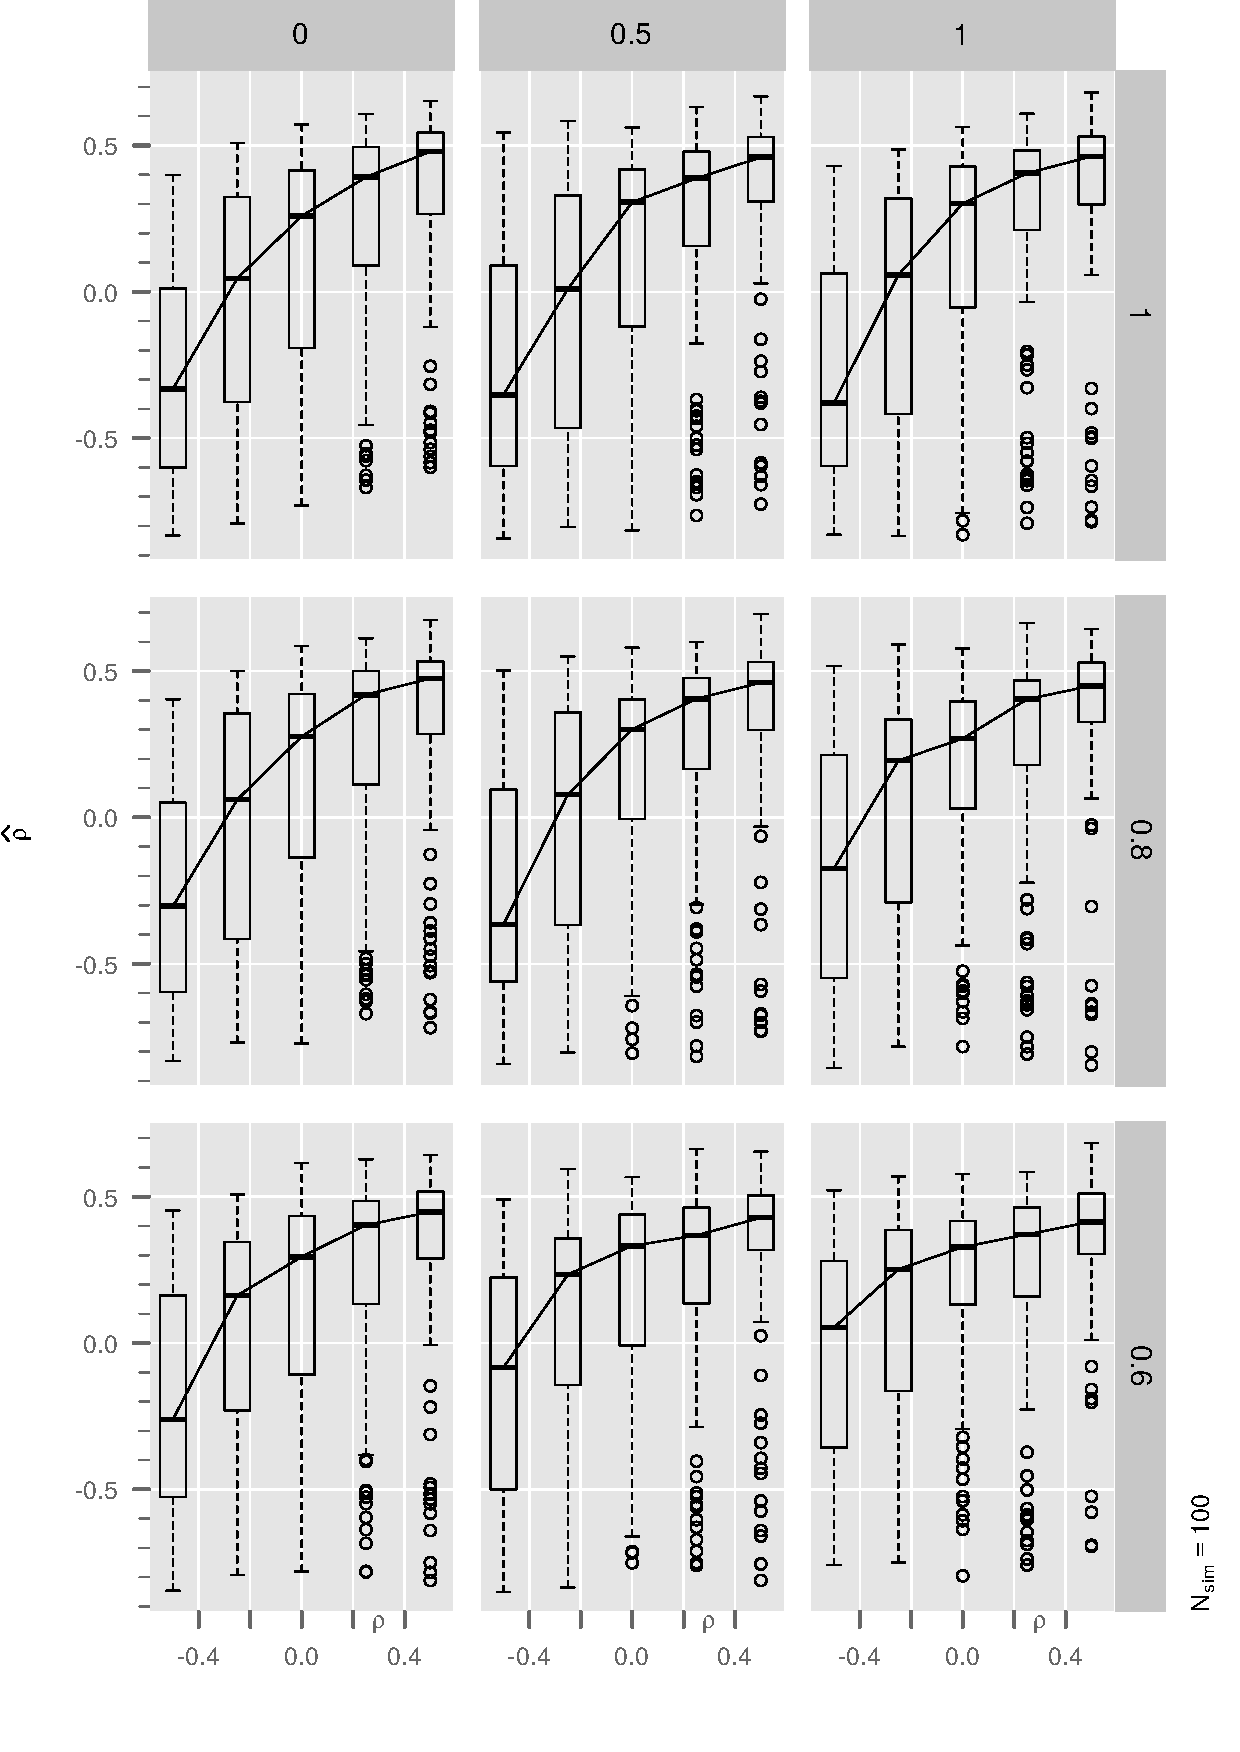
\includegraphics[trim= 0cm 0cm 0cm 11.75cm, clip, scale=0.475]{Figure1/tbl1_n100_rho_mayplot.pdf}
\end{center}

\end{frame}

\begin{frame}{1-sample: Correlation estimate, n=500 (Density plot)}

\begin{center}
  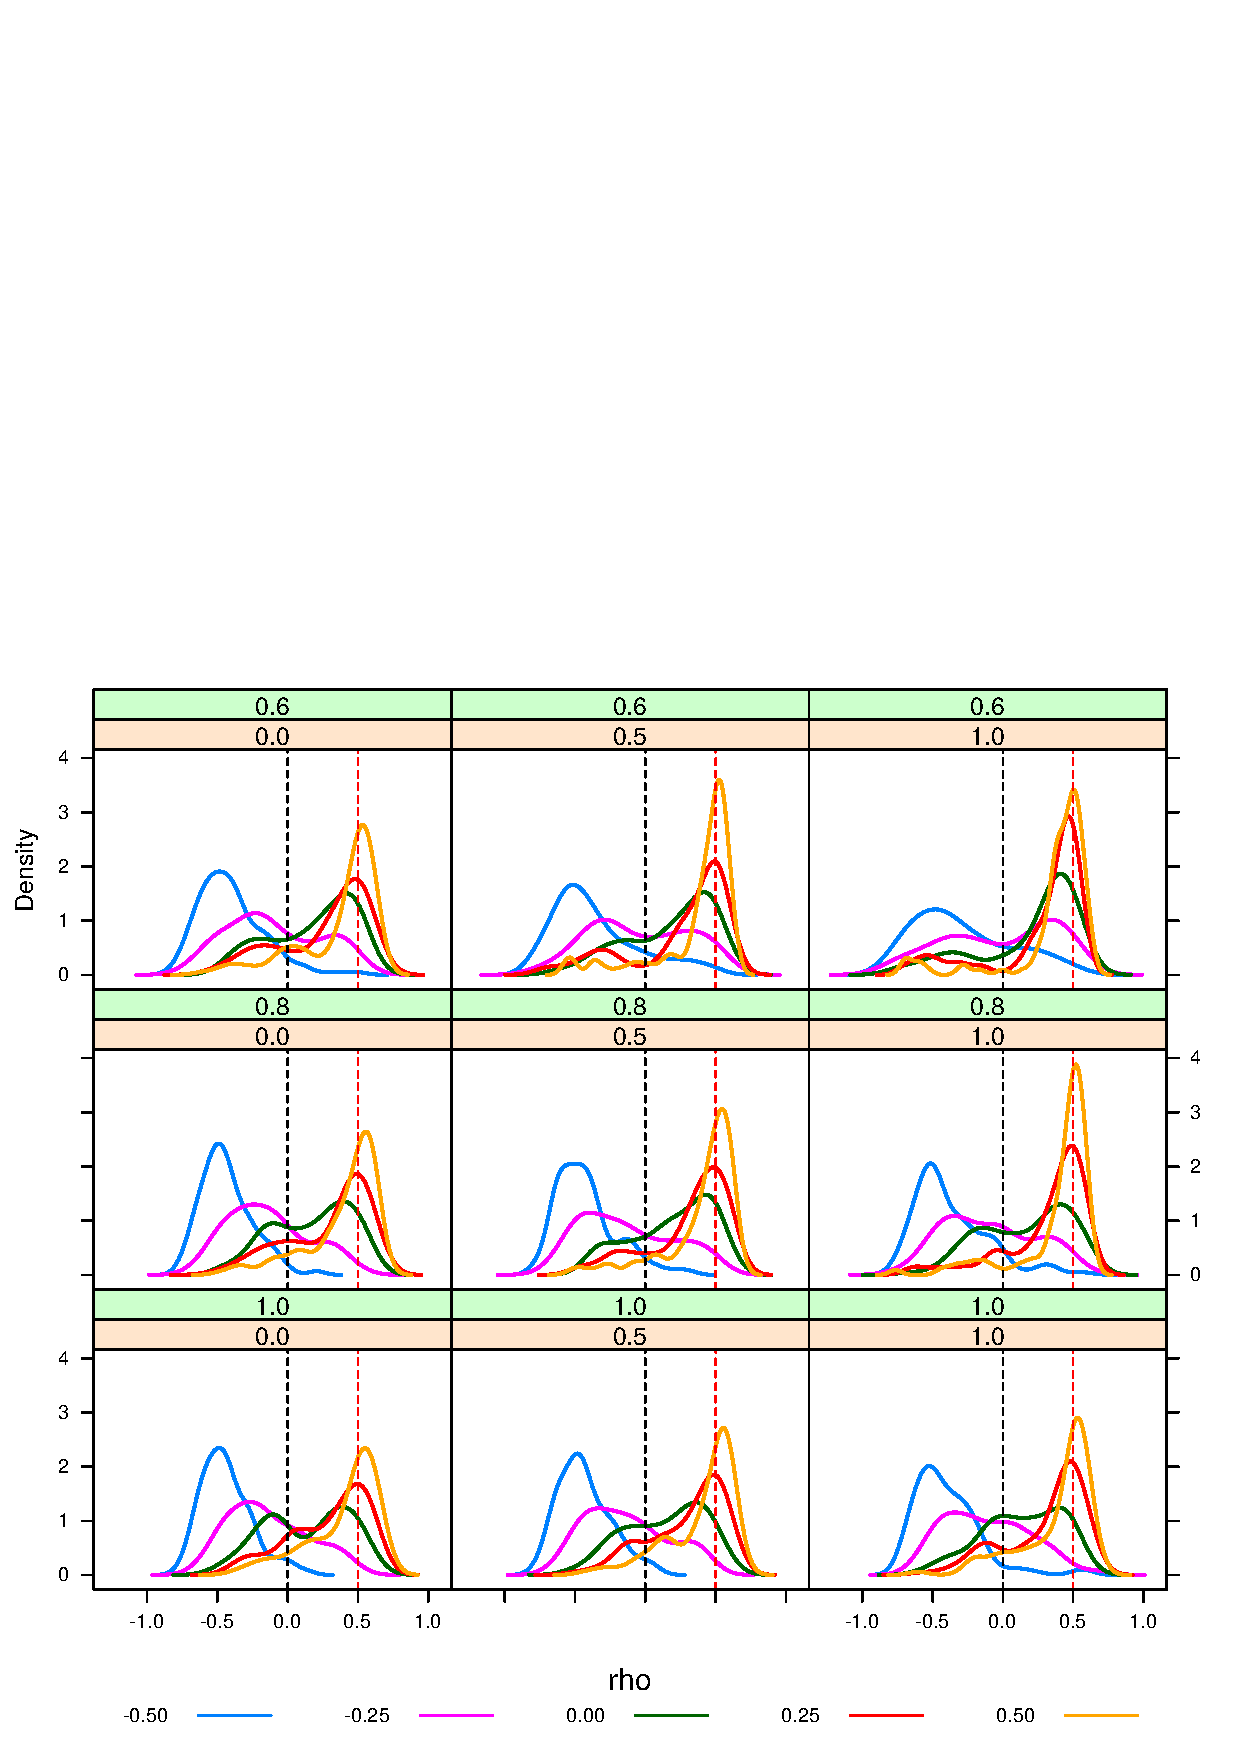
\includegraphics[trim= 0cm 0cm 0cm 11.75cm, clip, scale=0.47]{Figure1/tbl1densityPlot_n500.pdf} % width=1.00\textwidth, clip,, [scale=0.67]
\end{center}

\end{frame}

\subsection{2-sample: Estimation of treatment benefit}
\protect\hypertarget{two-samples}{}

\begin{frame}{2-sample: Treatment Benefit $\hat{\Delta}=\hat{\beta}_{21}$ (n=1000)} % 3b: n=1000
\begin{table}[htbp]
  \centering\scriptsize
  \begin{tabular}{*{2}{l}*{4}{r}}
    \toprule
     & beta12 & \multicolumn{2}{c}{0} & \multicolumn{2}{c}{1} \\
    \cmidrule(lr){3-4} \cmidrule(lr){5-6}
    cs & \( \rho \) \textbar\ deltaTreat & \multicolumn{1}{c}{0} & \multicolumn{1}{c}{0.5} & \multicolumn{1}{c}{0} & \multicolumn{1}{c}{0.5} \\
    \midrule
    1 & -0.5 & -0.00 & 0.50 & 0.00 & 0.51 \\
    & -0.25 & -0.00 & 0.48 & -0.01 & 0.50 \\
    & 0 & 0.00 & 0.46 & 0.00 & 0.50 \\
    & 0.25 & -0.01 & 0.49 & 0.00 & 0.49 \\
    & 0.5 & -0.00 & 0.52 & -0.00 & 0.49 \\ \addlinespace[3pt]
    0.8 & -0.5 & -0.00 & 0.50 & 0.00 & 0.50 \\
    & -0.25 & -0.00 & 0.48 & 0.01 & 0.49 \\
    & 0 & 0.01 & 0.49 & 0.00 & 0.49 \\
    & 0.25 & -0.00 & 0.48 & -0.01 & 0.48 \\
    & 0.5 & -0.01 & 0.51 & 0.01 & 0.51 \\ \addlinespace[3pt]
    0.6 & -0.5 & 0.02 & 0.49 & -0.01 & 0.48 \\
    & -0.25 & -0.02 & 0.52 & -0.00 & 0.48 \\
    & 0 & -0.01 & 0.49 & 0.01 & 0.48 \\
    & 0.25 & 0.02 & 0.49 & 0.01 & 0.50 \\
    & 0.5 & 0.00 & 0.51 & -0.01 & 0.51 \\
    \bottomrule
    \multicolumn{5}{l}{\footnotesize{medians of 100 replicates}} % \multicolumn{4}{l}{\textsuperscript{*}\footnotesize{The footnote}}
  \end{tabular}
%  \caption{b21 TreatDiff estimate: Table 3b, n=1000}
  \label{tab:ft21}
\end{table}

\end{frame}


%\begin{frame}{2-sample: Treatment Benefit, n=1000 (estimates)} % sf x beta12

%\begin{center}
%  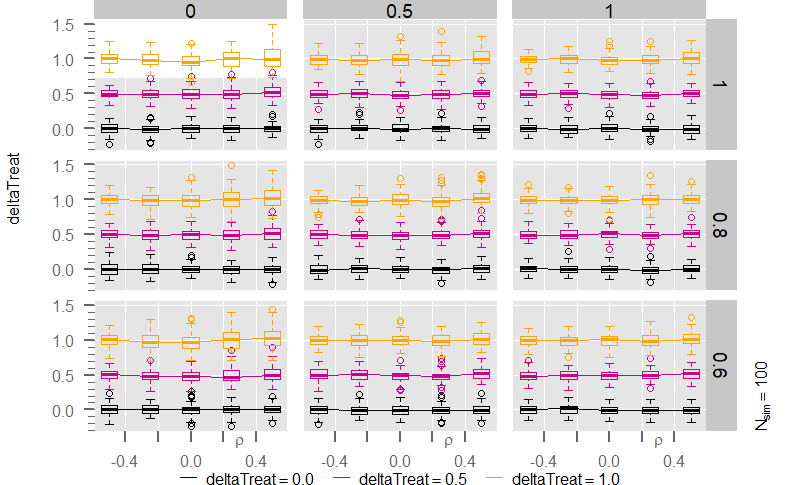
\includegraphics[width=1.00\textwidth]{Figure3/mayplot3-deltaTreat-n1000.png}
%\end{center}

%\end{frame}

%{Treatment Benefit, n=1000, sf=0.6 (density plots)}
%  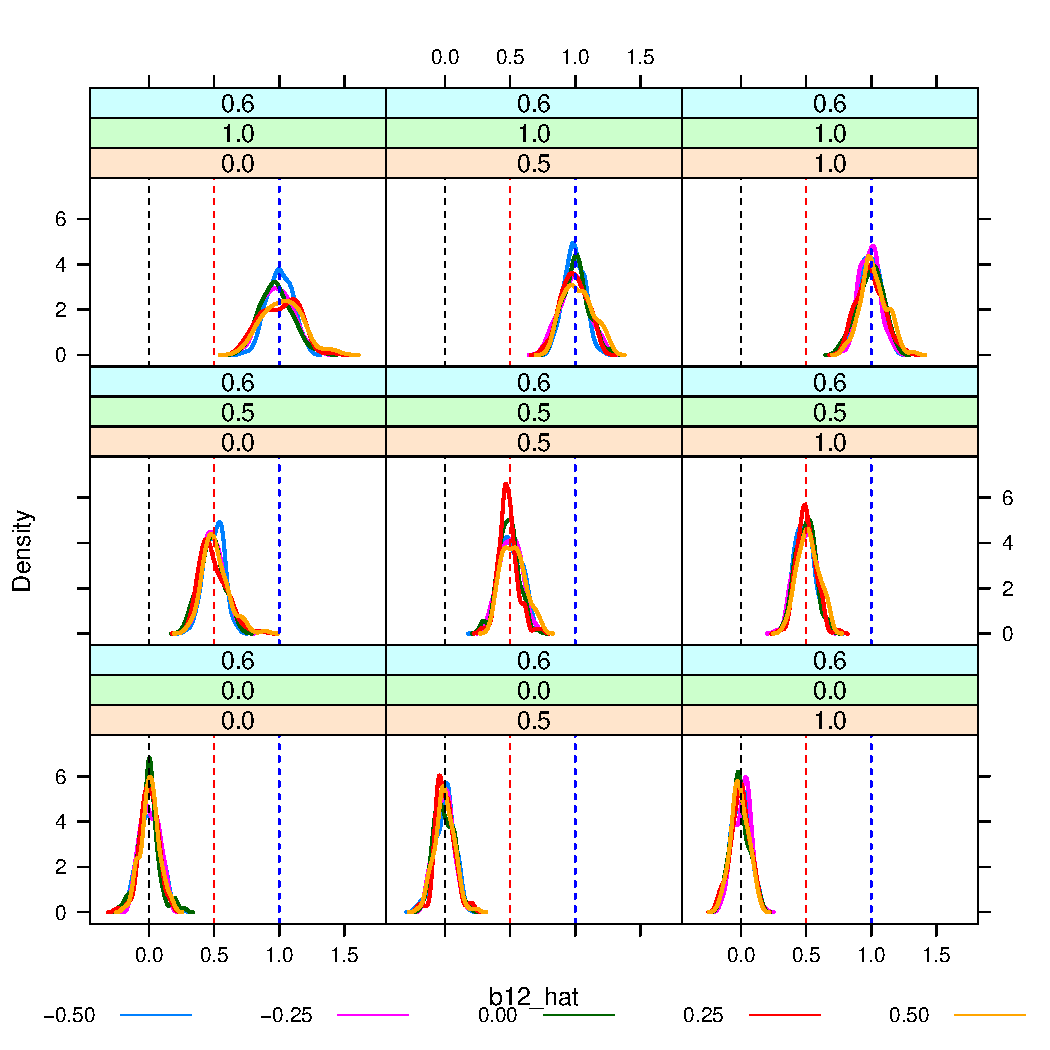
\includegraphics[scale=0.45]{Figure3/tbl3DensityPlots_n1000_003.pdf} % sf=0.6

\begin{frame}{2-sample: Treatment Benefit, n=100 (estimates)} % sf x beta12

\begin{center}
  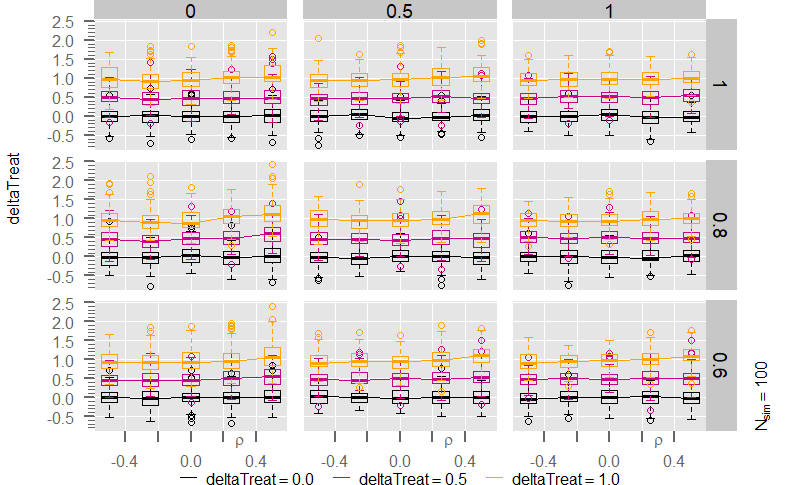
\includegraphics[width=1.00\textwidth]{Figure3/mayplot3-deltaTreat-n100.png}
\end{center}

\end{frame}

%  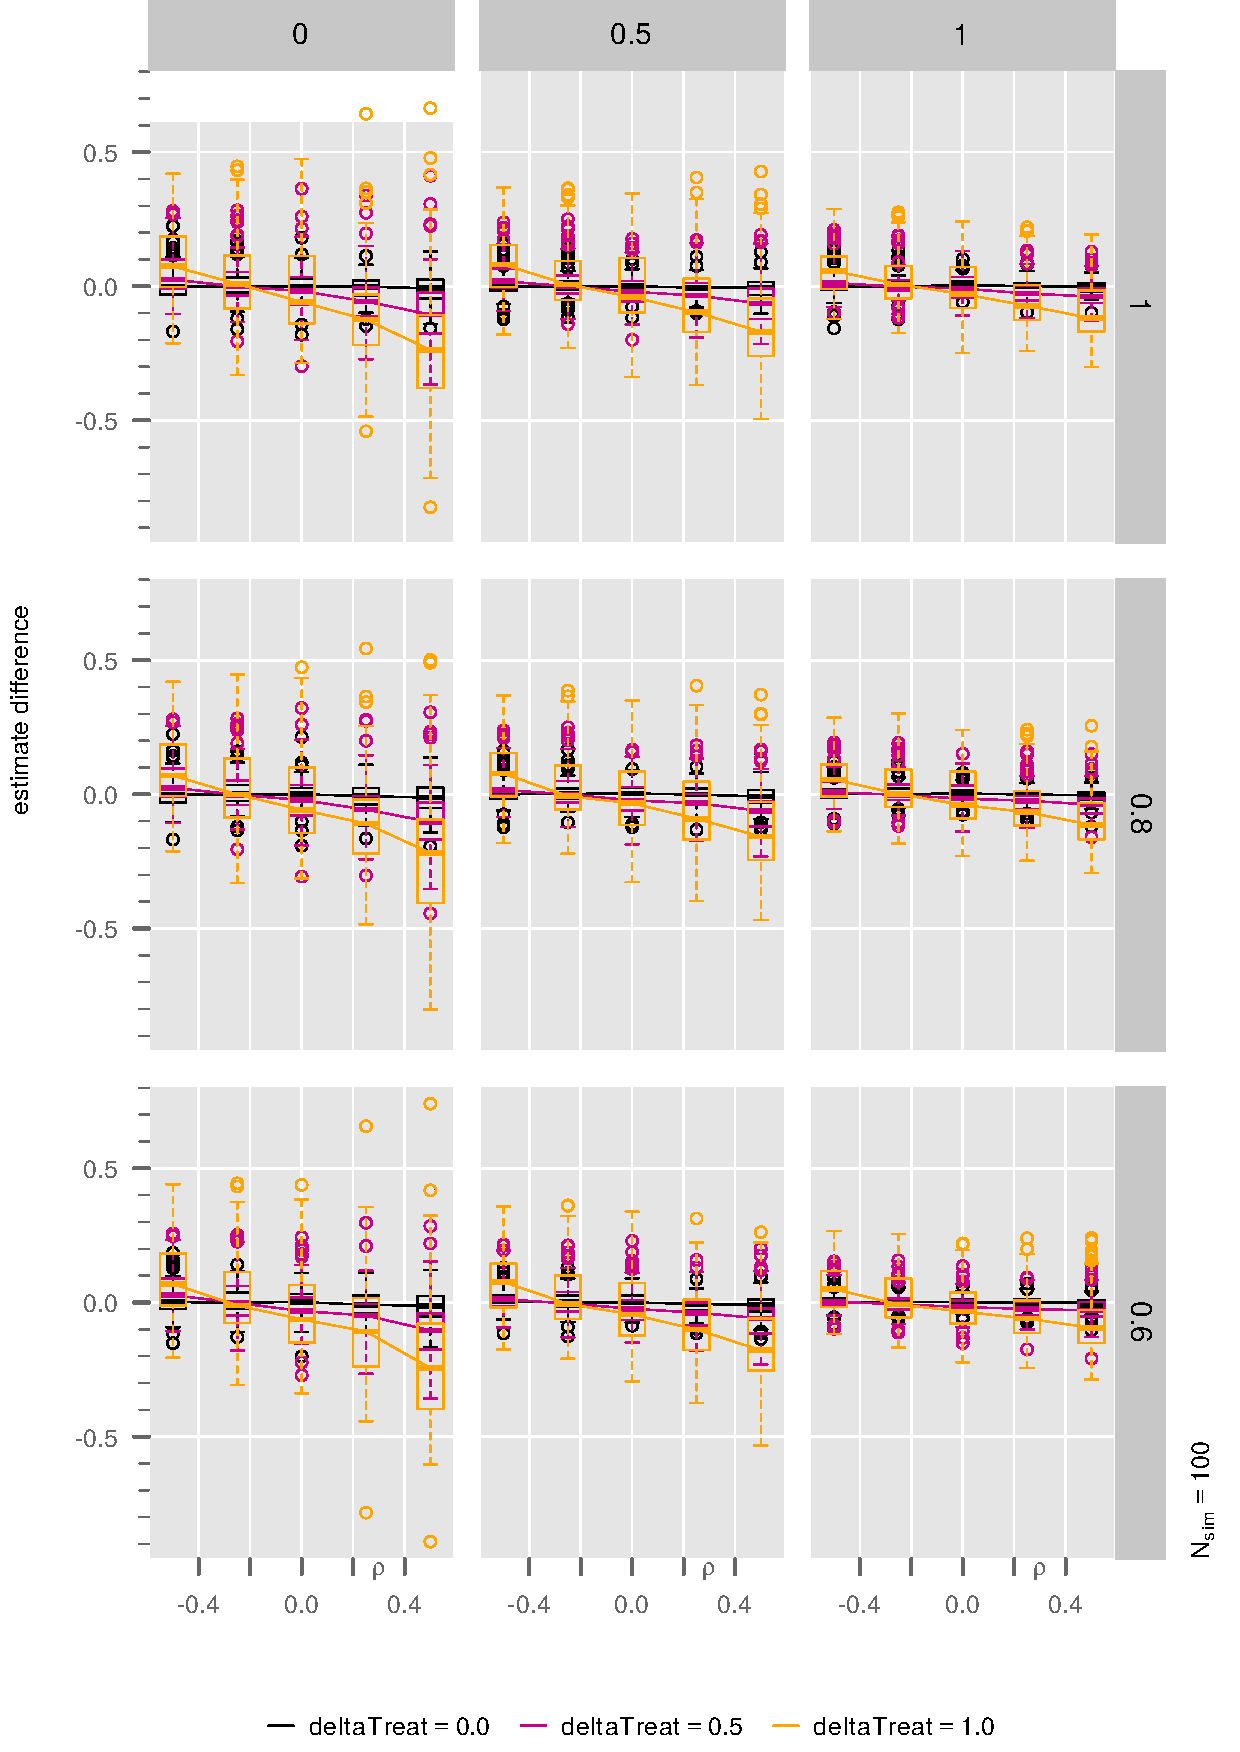
\includegraphics[width=0.95\textwidth]{Figure3/estimateDifferences2v12.pdf}

\begin{frame}{2-sample: survreg coef of treatment benefit ($\rho=0$), n=100}

\begin{center}
  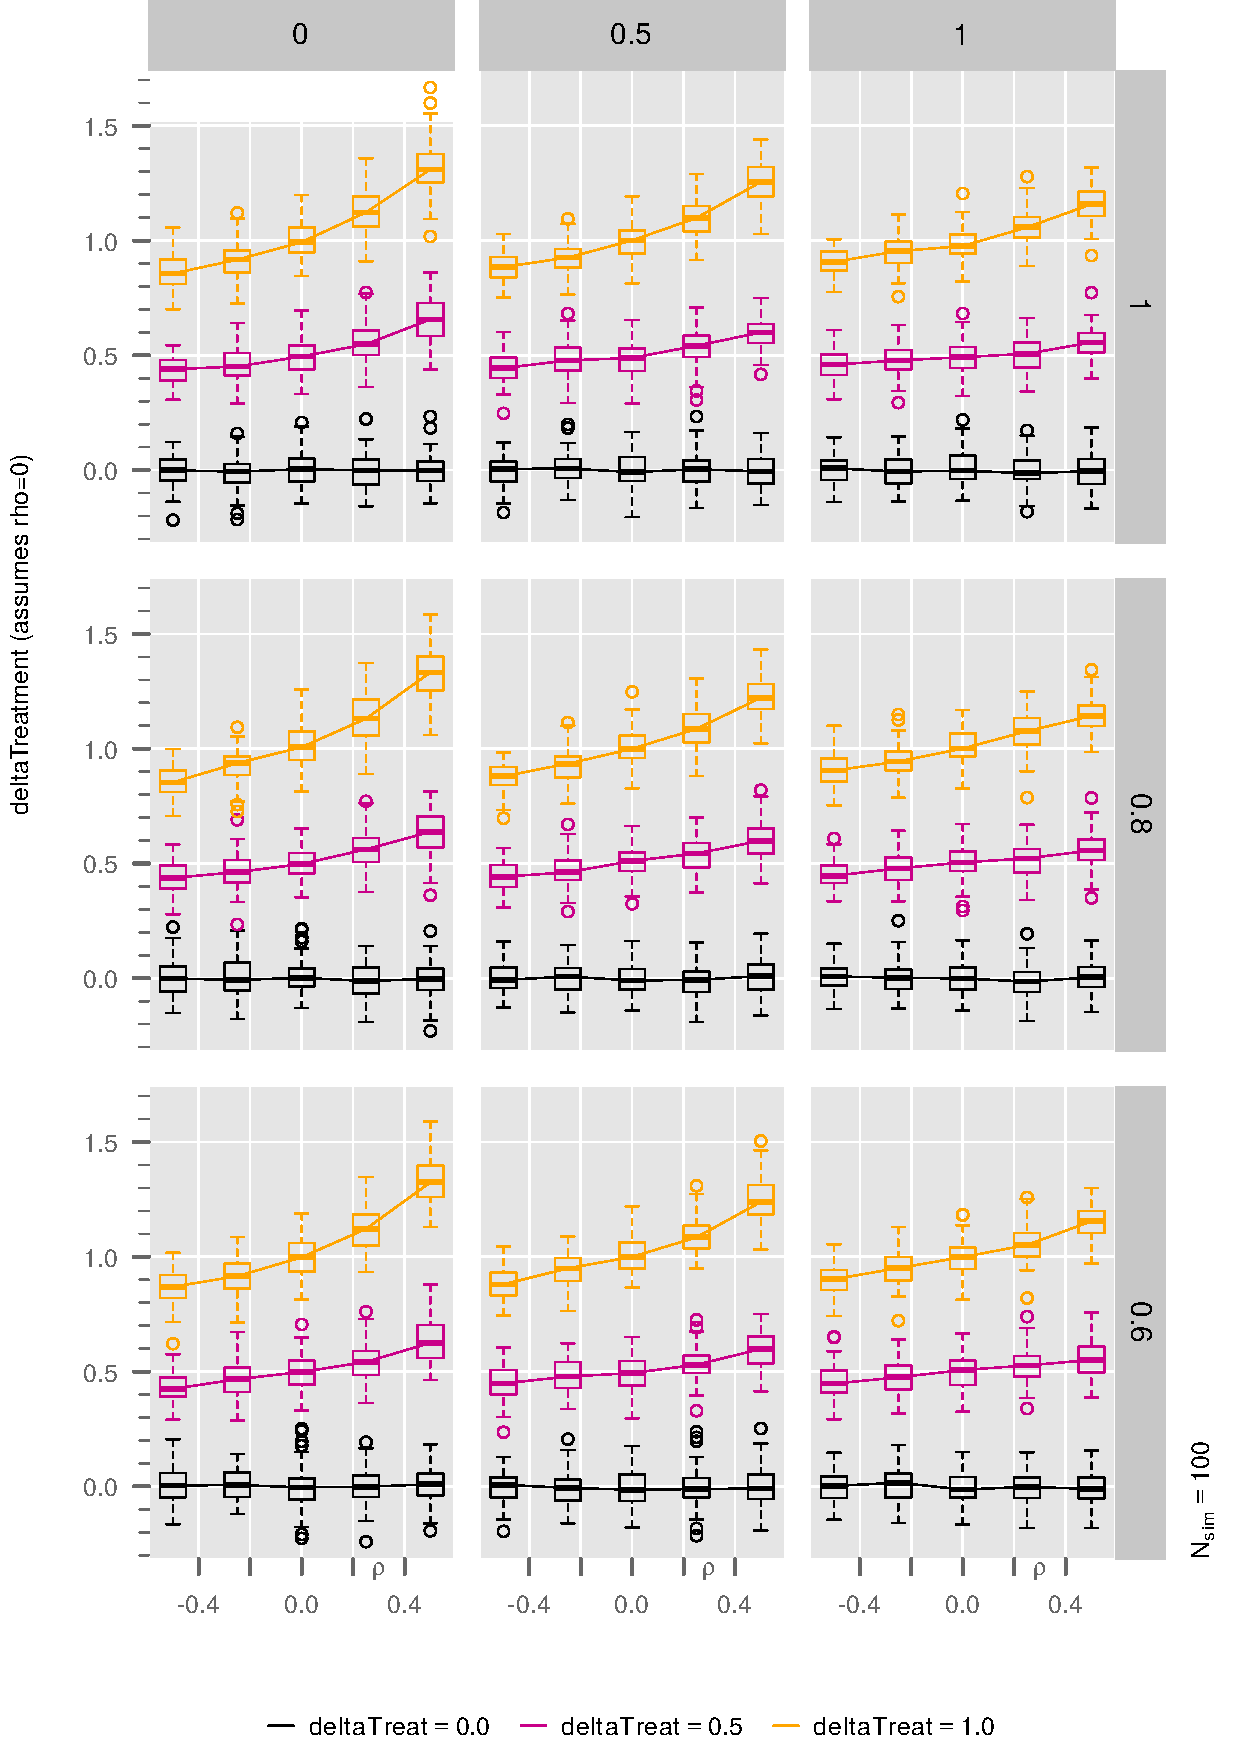
\includegraphics[width=1.00\textwidth]{Figure3/mayplot-coefTreat-n100-v2.pdf} % sf=0.6 scale=0.45
\end{center}

\end{frame}

%\begin{frame}{2-sample: Treatment difference: BNC estimate  vs survreg coef ($\rho=0$)}

%\begin{center}
%  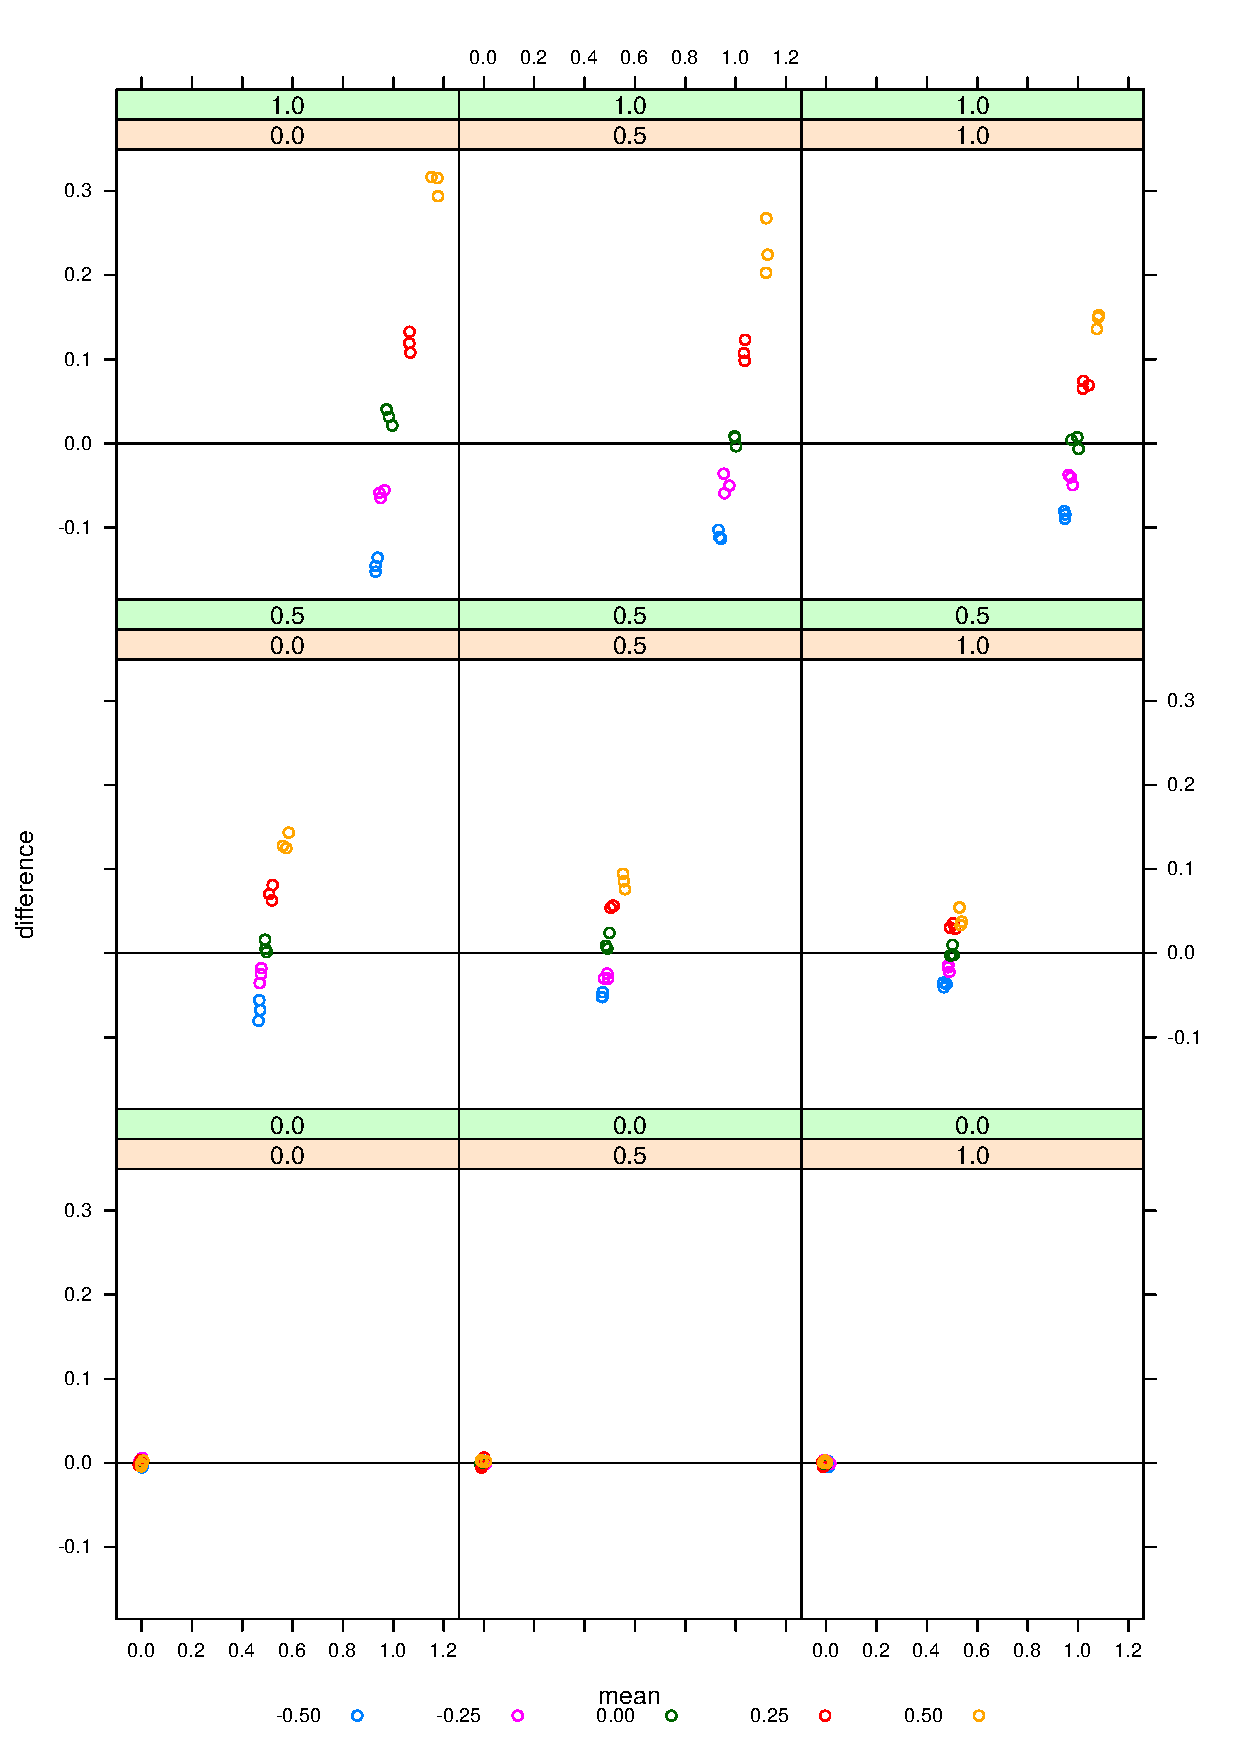
\includegraphics[height=0.95\textheight,width=0.95\textwidth]{%
%  Figure3/estimateDifferences2vs12v2.pdf%
%  }
%\end{center}

%\end{frame}


\begin{frame}{2-sample Treatment Benefit, n=1000, sf=0.6 (density plots)}

\begin{center}
  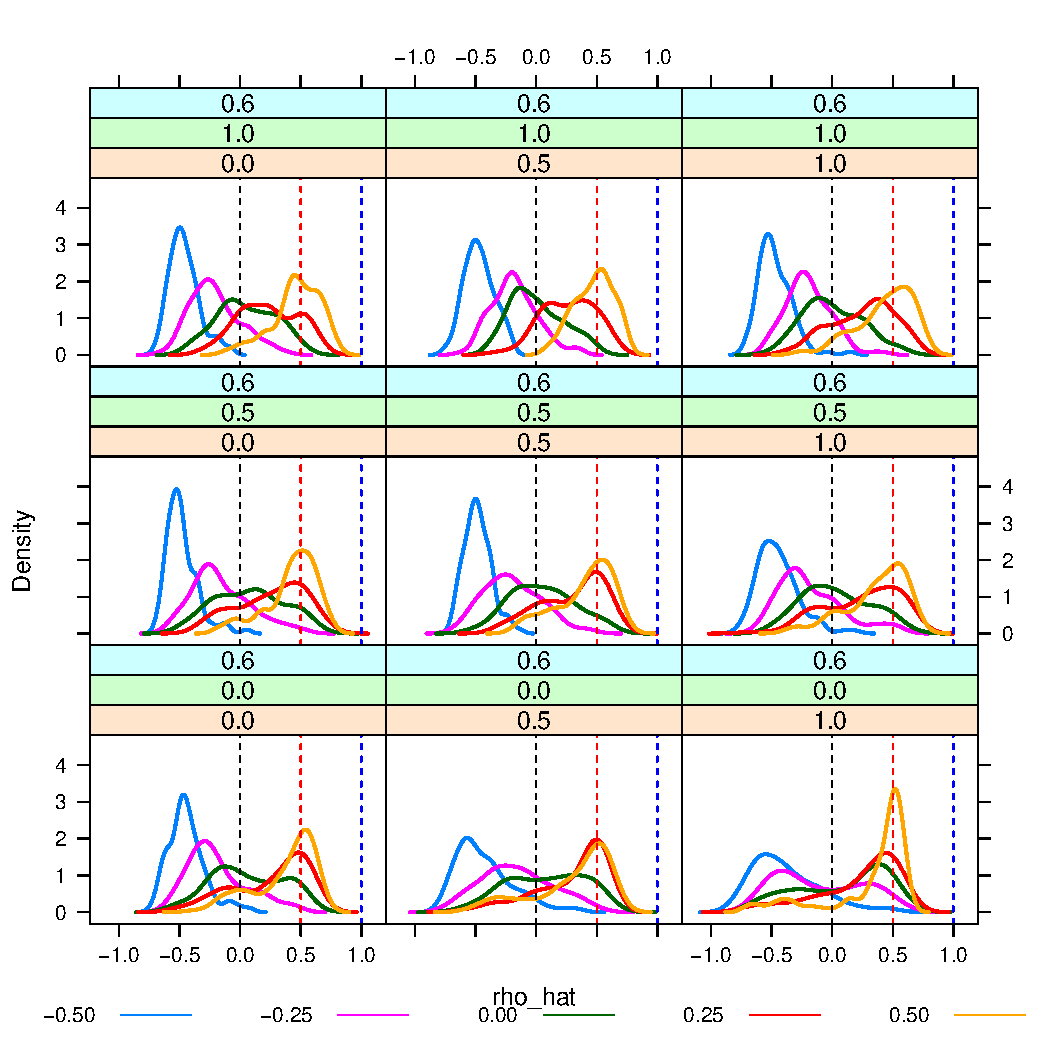
\includegraphics[scale=0.45]{Figure3/tbl3DensityPlots_rho_n1000_003.pdf} % sf=0.6
\end{center}

\end{frame}

\begin{frame}{3c: 2-sample  $\hat{\rho}$ (n=1000)  }
\begin{table}[htbp]
  \centering\scriptsize
  \begin{tabular}{*{2}{l}*{4}{r}}
    \toprule
     & beta12 & \multicolumn{2}{c}{0} & \multicolumn{2}{c}{1} \\
    \cmidrule(lr){3-4} \cmidrule(lr){5-6}
    cs & \( \rho \) \textbar\ deltaTreat & \multicolumn{1}{c}{0} & \multicolumn{1}{c}{0.5} & \multicolumn{1}{c}{0} & \multicolumn{1}{c}{0.5} \\
    \midrule
    1 & -0.5 & -0.50 & -0.49 & -0.51 & -0.51 \\
    & -0.25 & -0.24 & -0.22 & -0.23 & -0.25 \\
    & 0 & 0.05 & 0.07 & 0.12 & -0.02 \\
    & 0.25 & {\color{red}0.36} & 0.31 & {\color{red}0.37} & 0.31 \\
    & 0.5 & 0.49 & 0.49 & 0.51 & 0.50 \\ \addlinespace[3pt]
    0.8 & -0.5 & -0.50 & -0.49 & -0.48 & -0.50 \\
    & -0.25 & -0.20 & -0.22 & -0.16 & -0.24 \\
    & 0 & {\color{red}0.17} & 0.07 & {\color{red}0.10} & 0.02 \\
    & 0.25 & 0.31 & 0.27 & 0.25 & {\color{red}0.37} \\
    & 0.5 & 0.51 & 0.48 & 0.48 & 0.49 \\ \addlinespace[3pt]
    0.6 & -0.5 & -0.48 & -0.48 & -0.47 & -0.49 \\
    & -0.25 & -0.19 & -0.25 & -0.22 & -0.19 \\
    & 0 & 0.03 & 0.09 & {\color{red}0.14} & 0.05 \\
    & 0.25 & {\color{red}0.40} & 0.27 & {\color{red}0.44} & 0.27 \\
    & 0.5 & 0.53 & 0.50 & 0.46 & 0.51 \\
    \bottomrule
  \end{tabular}
  \caption{Correlation estimate (median, nsim=100): n=1000}
  \label{tab:ft3}
\end{table}

\end{frame}

